\section{Azure Function的持久化与存储(胡登杭)}\label{sec:serverless_DB}
\subsection{Durable Azure Functions}
Durable Functions 是 Azure Functions 的一个扩展,可用于在无服务器计算环境中编写有状态函数。  
有几种典型的应用模式:
\subsubsection{模式 1:函数链}
如图\ref{fig:model1}所示,在函数链接模式中,将按特定顺序执行一系列函数。 在此模式中,一个函数的输出将应用到另一函数的输入。
\begin{figure}[!htbp]
	\centering
	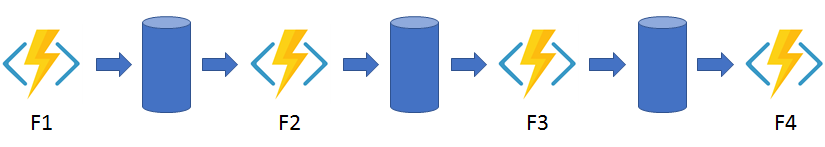
\includegraphics[width=0.8\linewidth]{figs/model1}
	\caption{函数链(\cite{Durable})}
	\label{fig:model1}
\end{figure}

\subsubsection{模式 2:扇出/扇入}
如图\ref{fig:model2-3}(a)所示,在扇出/扇入模式中,将会并行执行多个函数,然后等待所有函数完成。 通常会对这些函数返回的结果执行一些聚合操作。
\begin{figure}[!htbp]
	\begin{subfigure}[b]{0.62\linewidth}
		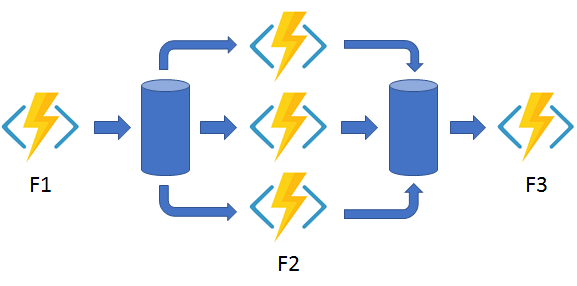
\includegraphics[width=\linewidth]{figs/model2}
		\caption{}
	\end{subfigure}
	\begin{subfigure}[b]{0.38\linewidth}
		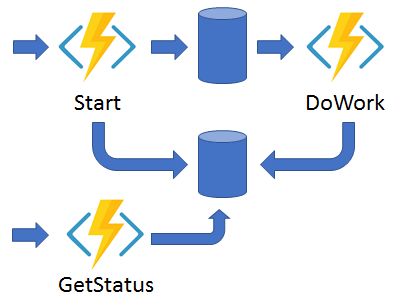
\includegraphics[width=\linewidth]{figs/model3}
		\caption{}
	\end{subfigure}
	\caption{(a) 扇出/扇入。(b) 异步 HTTP API。(\cite{Durable})}
	\label{fig:model2-3}
\end{figure}

\subsubsection{模式 3:异步 HTTP API}
如图\ref{fig:model2-3}(b)所示,异步 HTTP API 模式解决了使用外部客户端协调长时间运行的操作的状态时出现的问题。 实现此模式的一种常用方式是让 HTTP 终结点触发长时间运行的操作。 然后,将客户端重定向到某个状态终结点,客户端可轮询该终结点,以了解操作是何时完成的。

\subsubsection{模式 4:监视}
如图\ref{fig:model4-6}(a)所示,监视模式是指工作流中的灵活重复进程。 例如,轮询到满足特定的条件为止。 可以使用常规计时器触发器解决简单方案(例如定期清理作业),但该方案的间隔是静态的,并且管理实例生存期会变得复杂。 可以使用 Durable Functions 创建灵活的重复间隔、管理任务生存期,以及从单个业务流程创建多个监视进程。
监视模式的一个例子是反转前面所述的异步 HTTP API 方案。 监视模式不会公开终结点供外部客户端监视长时间运行的操作,而是让长时间运行的监视器使用外部终结点,然后等待某个状态发生更改。

\subsubsection{模式 5:人机交互}
如图\ref{fig:model4-6}(b)所示,许多自动化过程涉及到某种人机交互。 自动化过程中涉及的人机交互非常棘手,因为人的可用性和响应能力不如云服务那样高。 自动化过程允许使用超时和补偿逻辑来实现这种交互。
审批过程就是涉及到人机交互的业务过程的一个例子。 例如,某份超出特定金额的开支报表需要经理的审批。 如果经理未在 72 小时内审批该开支报表(经理可能正在度假),则会启动上报过程,让其他某人(可能是经理的经理)审批。
\begin{figure}[!htbp]
	\begin{subfigure}[b]{0.28\linewidth}
		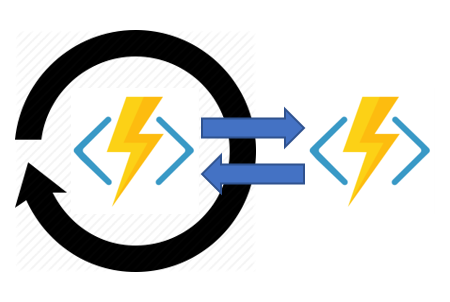
\includegraphics[width=\linewidth]{figs/model4}
		\caption{}
	\end{subfigure}
	\begin{subfigure}[b]{0.36\linewidth}
		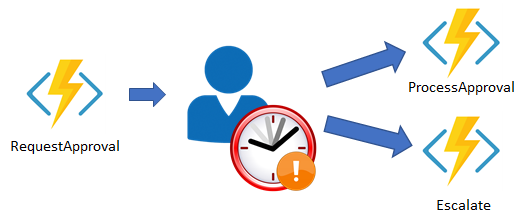
\includegraphics[width=\linewidth]{figs/model5}
		\caption{}
	\end{subfigure}
	\begin{subfigure}[b]{0.36\linewidth}
		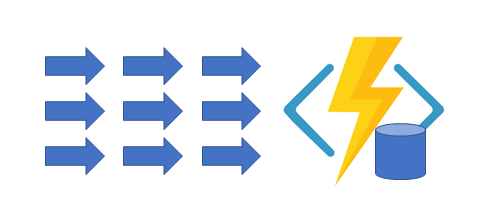
\includegraphics[width=\linewidth]{figs/model6}
		\caption{}
	\end{subfigure}
	\caption{(a) 监视。(b) 人机交互。(c) 聚合器。(\cite{Durable})}
	\label{fig:model4-6}
\end{figure}

\subsubsection{模式 6:聚合器(有状态实体)}
如图\ref{fig:model4-6}(c)所示,第六种模式涉及到将一段时间的事件数据聚合到单个可寻址的实体。 在此模式中,要聚合的数据可来自多个源、可分批传送,也可以分散在较长的时间段。 聚合器可能需要在事件数据抵达时对其执行操作,而外部客户端可能需要查询聚合数据。

\subsection{Azure Data Lake Store}
\subsubsection{Azure Data Lake Analytic}
Azure Data Lake Store(ADLS) 是微软针对Azure Data Lake Analytic(ADLA)研发的一套存储系统。所以在了解ADLS之前,我们先了解一下ADLA.\\
Data Lake, 中文翻译为数据湖。五湖四海,海纳百川,湖泊象征着广博,象征着纷繁复杂。所以顾名思义数据湖代表一类没有经过处理的、杂乱的原始数据。为了提取出数据中的有效信息,所以需要对数据湖进行"analytic",这就是Data Lake Analytic的含义。然而由于数据湖中的数据是原始的、未经过处理的,所以数据量会非常大,现代数据湖的数据量已经到了EB量级。为了能够分布式地存储和分析这么大量级的数据,微软研发了分布式存储系统ADLS。
\subsubsection{设计目标}
ADLS主要是为ADLA服务的,主要的设计目标跟数据湖分析的目标相似,有三点:1)处理高并发的读操作和写操作;2)低延时地处理高带宽的数据;3)存储大量数据(EB量级)。
\subsubsection{设计特色}
ADLS和HDFS一样是分布式存储系统,是Cosmos存储系统的一个延伸,它综合了HDFS和Cosmos存储系统优点。主要有两个特色:支持多种存储方式和特殊的文件存储方式。
\begin{figure}[!htbp]
	\begin{subfigure}[b]{0.5\linewidth}
		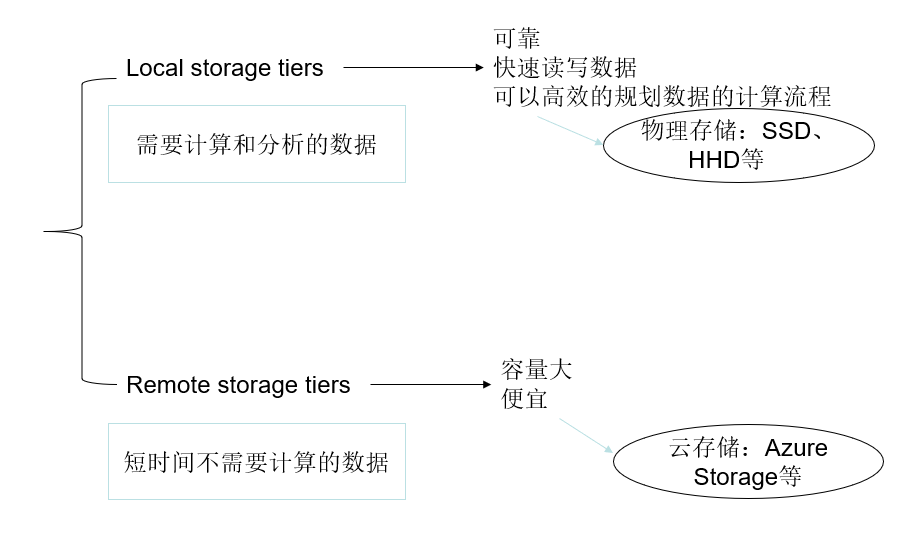
\includegraphics[width=\linewidth]{figs/data_store.png}
		\caption{}
		\label{fig:data_store}
	\end{subfigure}
	\begin{subfigure}[b]{0.5\linewidth}
		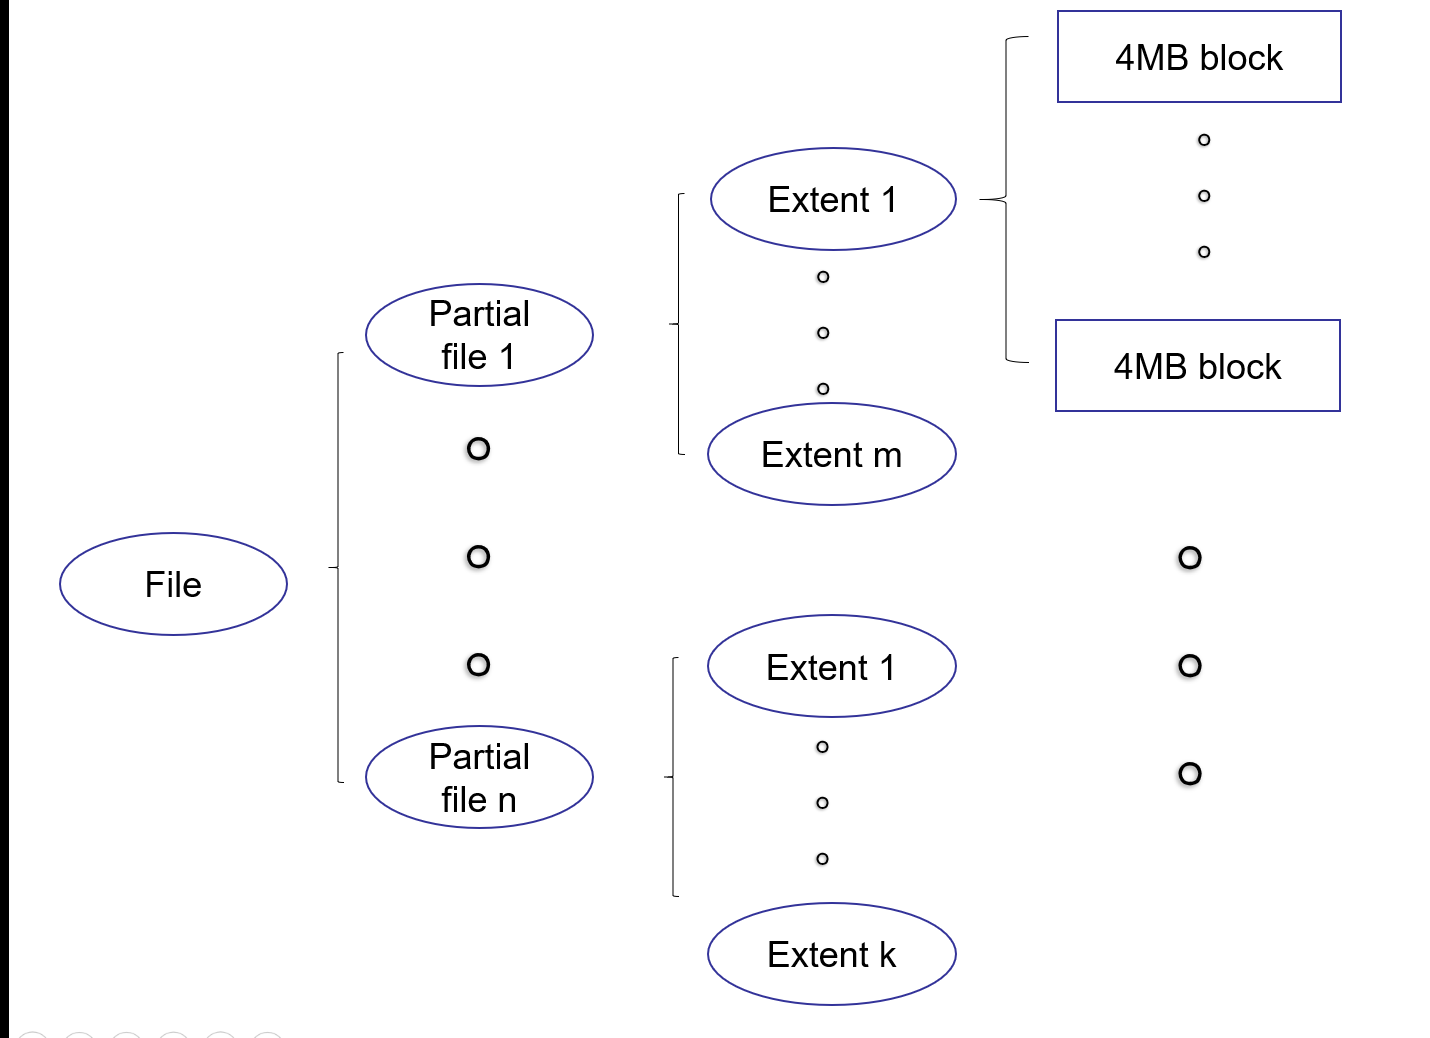
\includegraphics[width=0.8\linewidth]{figs/file_store.png}
		\caption{}
		\label{fig:file_store}
	\end{subfigure}
	\caption{(a) ADLS存储的两种方式:local storage tiers和remote storage tiers。(b) ADLS文件设计的方式:把一个文件细分为partial file,每个partial file又细分为extents,每个extents由基本的4KB的数据块组成。}
\end{figure}
\begin{enumerate}
	\item \textbf{支持多种存储方式-物理存储和云存储}\ \ ADLS把存储系统抽象为Storage tiers, 每个tiers对应着一个特有的存储提供商。存储提供商可以是本地的物理存储如SSD,也可以是云存储如Azure Storage。如\ref{fig:data_store}所示,Storage tiers分为两种类型:Local storage tiers和 Remote storage tiers。
	\begin{itemize}
		\item Local storage tiers:本地存储层中的数据直接存储在ADLS内部节点中,如本地计算机的SSD中。这些数据可以被ADLS快速的访问,在做计算任务时也容易规划。所以一般把短时间内需要频繁计算和分析的数据放在本地存储层。
		\item Remote storage tiers:然而本地存储层的容量总是有限的,为了处理EB量级的数据,还需要借助其他云存储服务器的空间,称为远端存储层。远端存储层数据的访问较慢,数据通信较慢导致计算速度也慢,唯一的优点就是空间大。一般用来存储短时间不需要分析的数据。
	\end{itemize}
	\item \textbf{把每个文件分段存储}\ \ 如\ref{fig:file_store}所示,ADLS把每个文件细分为了partial file, 对每个partial file又细分为了extents,每个extents由多个4KB的数据块组成;目的是便于维护分布式读写操作的正确性。每个file、partial file和extent都有sealed和unsealed两个状态,定义如下:
	\begin{itemize}
		\item Sealed extent: 该extent只读。
		\item Unsealed extent: 该extent可以追加写(append)。
		\item Sealed partial file: 该partial file只读。
		\item Unsealed partial file: 该partial file可以追加写。
		\item Sealed file: 该文件不可追加写,但是可以调整partial file的顺序,对partial file进行合并和分裂。
		\item Unsealed file:可以追加写。
	\end{itemize}
	ADLS保证任意时刻任何文件都只有一个unsealed partial file, 称为tailed partial file。在这个Unsealed partial file中只有一个unsealed extent, 称为tailed extent。这样的做法可以简化append操作的并发控制流程,而且能够有效的减少I/O,因为每次修改文件时不用读取整个文件,只用读取tailed extent。而且同一文件的partial file在任何时候都可以进行重排、分裂和合并。这样可以让ADLS在对文件进行append和concatenation操作时更加高效。
\end{enumerate}

\subsubsection{ADLS架构}
了解了ADLS的基本存储和文件的设计,我们再来看一看ADLS的整体架构,如图\ref{fig:ADLS-arc}所示。架构图\ref{fig:ADLS-arc}主要分为三部分:最左边这一部分(Centerlized, highly available micro-services)主要是各种微型服务器,比如给新建文件命名的Naming Service(NS), 管理extent状态的Extent Management Service(EMS)和管理partial file的 Partial File Manager(PFM);下边部分(ADLS Back End Cluster)是存储文件的服务器,这个服务器可以是本地的SSD,也可以是云服务器如Cosmos和Azure Storage;上边部分(ADLS GateWay Cluster)主要给用户提供创建、修改和删除文件等操作的API,其中核心的部分是Secure Store Service(SSS)。在用户发出一个文件操作后,SSS会询问微服务器如NS、EMS和PFM得到文件的具体信息如元数据,然后再去ADLS Back End Cluster对文件做相应的操作。
\begin{figure}[!htbp]
	\centering
	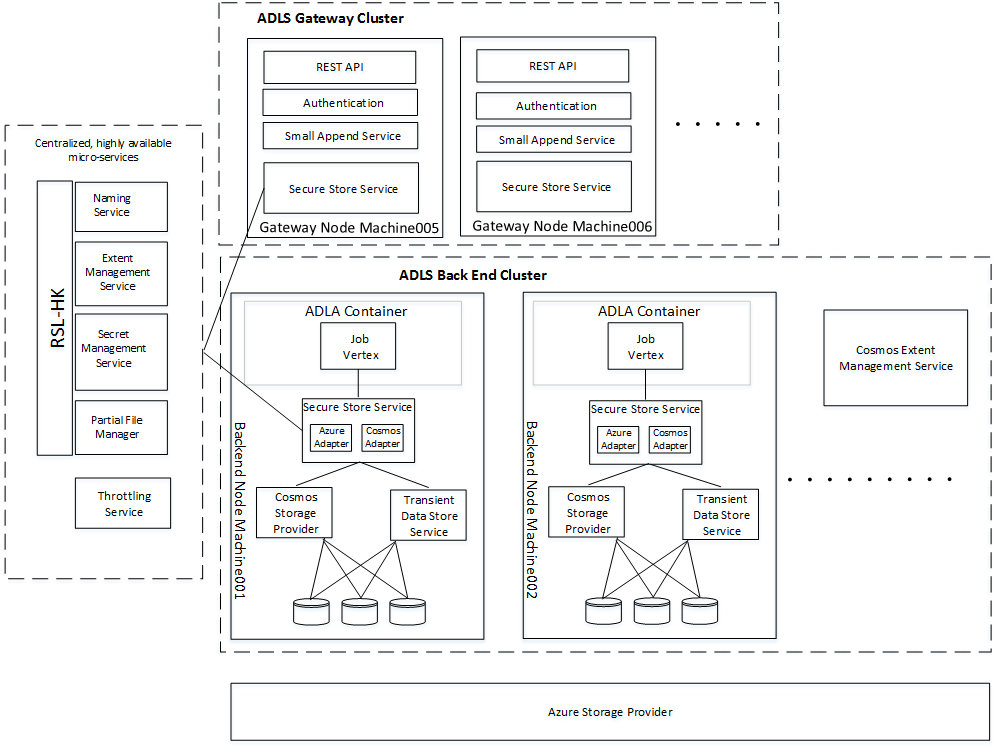
\includegraphics[width=0.78\linewidth]{figs/ADLS-arc.png}
	\caption{ADLS的架构图,主要由三部分组成:micro-services,ADLS Back End Cluster和ADLS GateWay Cluster,其中最核心的控制部分是Secure Store Service。(\cite{ramakrishnan2017azure}图2-2)}
	\label{fig:ADLS-arc}
\end{figure}

ADLS主要支持五种基本的文件操作,open、append、read、concatenation、enumeration。这些操作基于ADLS独特的文件系统设计(partial file和extent),有些操作会变得异常高效:如append只用取一个extents来进行修改,减少了大文件的I/O;concatenation 甚至不用文件I/O,只用在NS和PFM中做修改。操作的具体流程如下:\\
\textbf{open:} 
open是为了之后的文件操作,主要的目的是拿到保留在PFM中的tailed partial file ID和provider中的tailed extents ID。
\begin{itemize}
	\item 创建一个文件:Secure Store Service(SSS)在Naming Service(NS)中创建一个索引。SSS选择一个 存储提供商 (如Azure Storage)存储tail partial file,并在Partial File Manager(PFM)中创建一个索引。SSS请求存储提供商创建一个文件。
	\item 打开一个文件:SSS在NS索引中搜索文件得到File ID。SSS在PFM索引中搜索File ID得到Provider ID和tailed partial file ID。
\end{itemize}
\textbf{append:}
\begin{itemize}
	\item fixed-offset append:用户确定数据在文件中的偏移。如果文件中该偏移下有数据,操作异常中止。
	\item free offset append:ADLS自动设置文件偏移,加在文件末尾。
\end{itemize}
\textbf{read:}
\begin{itemize}
	\item Specifying a byte range to read:数据可能同时在多个存储提供商上存储,SSS选择最快的读。
	\item Access extents directly:先得到文件的元数据,然后通过元数据去寻找对应的extent。
\end{itemize}
\textbf{concatenation:}把多个文件连成一个文件。只需要修改NS和PFM中的索引即可。\\
\textbf{enumeration:}返回文件长度和最近修改时间。如果文件是sealed,那么只用访问PFM就行。如果文件是unsealed,SSS会询问存储tailed partial file的存储提供商以得到具体信息。

